%!TEX root =  ../main.tex

\mychapters{Triangles}{triangles}{\chapdir/pics/Northern_lights_in_Greenland} 

Amazingly, the trigonometric functions defined by right-triangles are
meaningful on non-right triangles.  The Pythagorean theorem is actually
just a special case of the Law of Cosines.  Triangles, it seems, are the
building blocks of the universe.

Why are triangles so productive?  What is so special about triangles?
Is there another shape with such descriptive power?

\newpage
\chapterminitoc


%									11 - 1
\newpage
\section{Area Formulae}
\noindent\makebox[\textwidth]{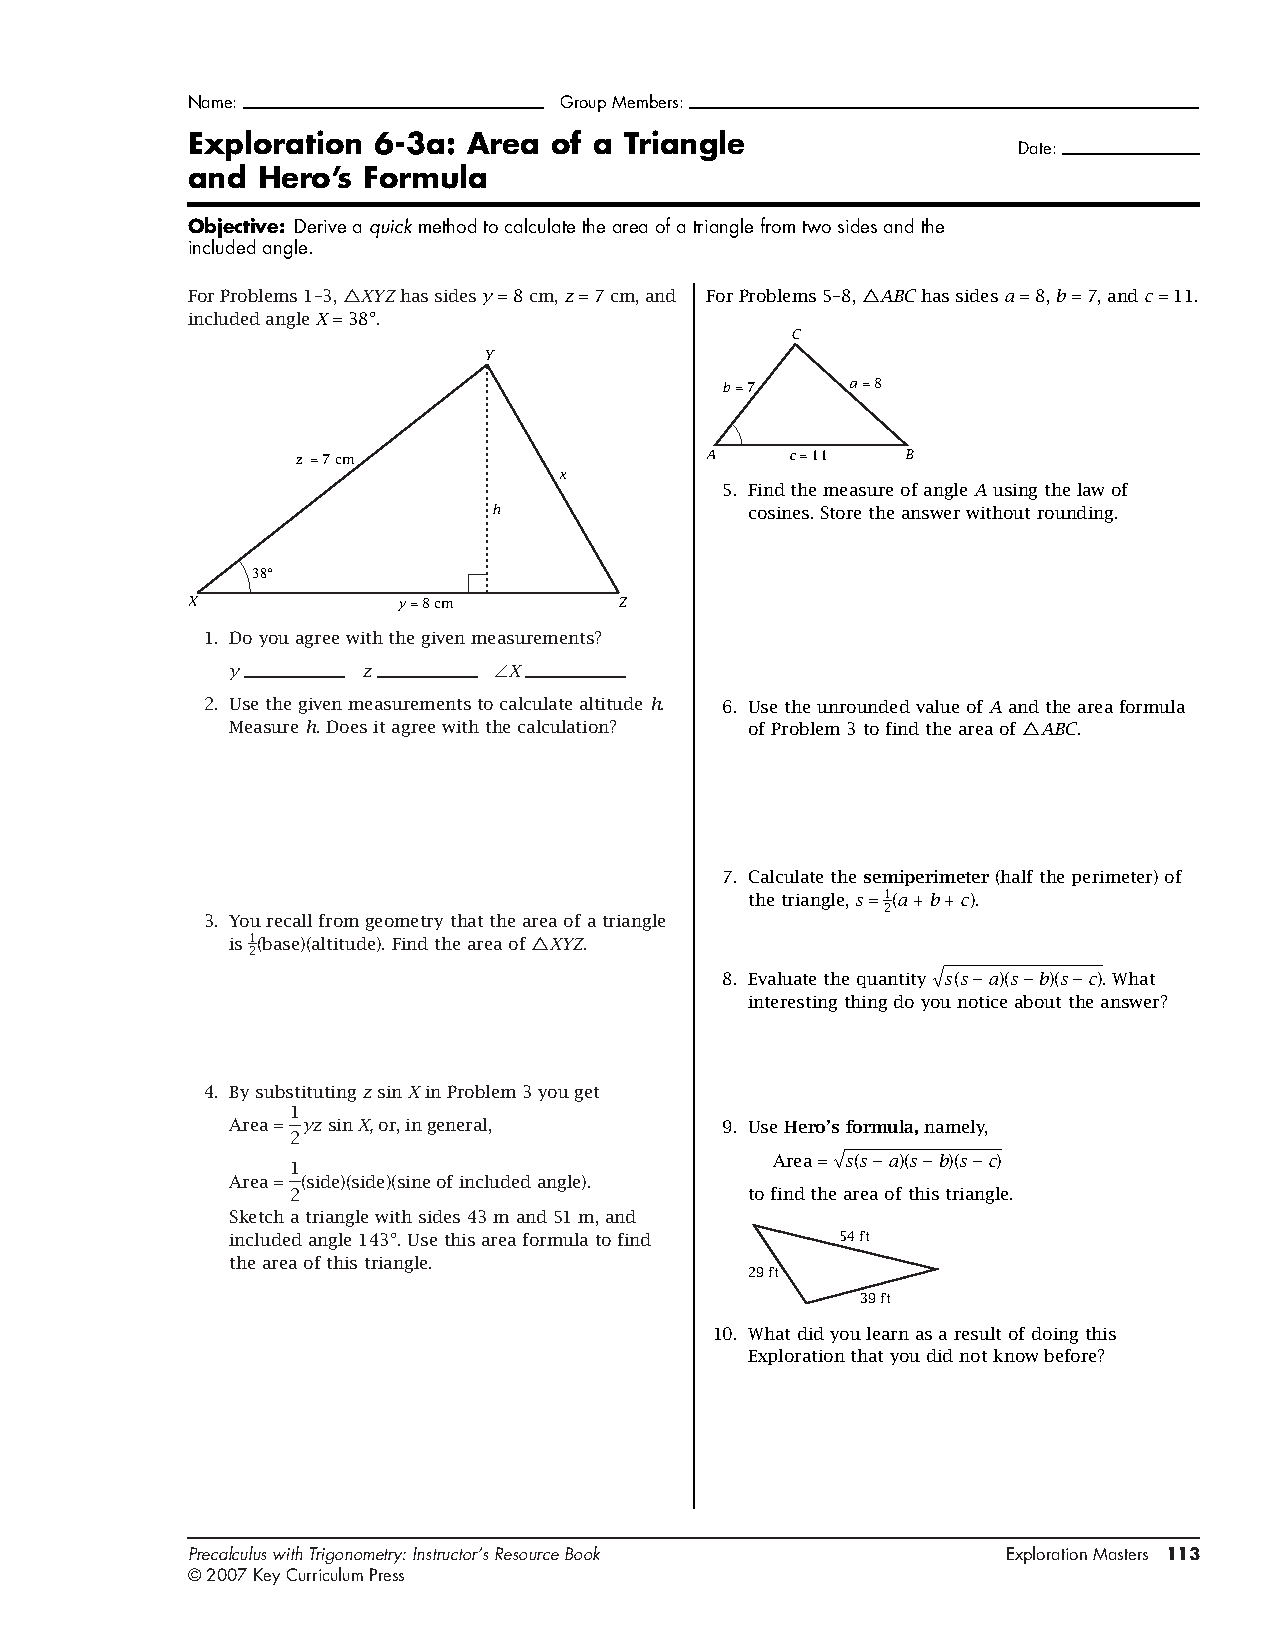
\includegraphics[width=\paperwidth]{ch11/1101p.pdf}}
\subsection{Sine Formulae}
Every child with any years under his or her belt in school knows that the area of a triangle is
$\frac{1}{2}bh$.  But what if we don't know $h$, the height?  It turns out, other information
is just as good.

Consider a triangle with side $b$ on the bottom.  For convenience's sake, we will put angle
A on the left, angle C on the right, and have angle B above.  If we drop an altitude from angle
C onto side $b$, we have $h$, and have bisected ABC into two right triangles.  We see,
therefore, that $\sin A = \frac{h}{c}$ and that $\sin C = \frac{h}{a}$.  Solving both equations
for $h$, we see that $h = c \cdot \sin A = a \cdot \sin C$.  If we don't know $h$ and we want to
find the area, we can substitute in either of these expressions.  This procedure would also have
worked for the other rotations of triangle ABC.

\begin{equation}
\text{the area of triangle ABC} = \frac{1}{2} a \cdot b \cdot \sin C = \frac{1}{2} a \cdot \sin B \cdot c = \frac{1}{2} \sin A \cdot b \cdot \sin C
\end{equation}

\subsection{Heron's Formula}
While the proof is very lengthy, the ancient Greek mathematician Hero proved that the area of a 
triangle is related to itself \textbf{semi-perimeter}, that is, half the total length around the outside.
If we have some triangle with sides $a$, $b$, and $c$, then $s = \frac{a + b + c}{2}$.  

\begin{equation}
\text{the area of a triangle ABC} = \sqrt{s(s-a)(s-b)(s-c)}
\end{equation}

\newpage
\subsection{Exercises}
To be done in Kuta


%									11 - 2
%\newpage
\invisiblesection{Law of Cosines}
\subsection{Problems}
\noindent\makebox[\textwidth]{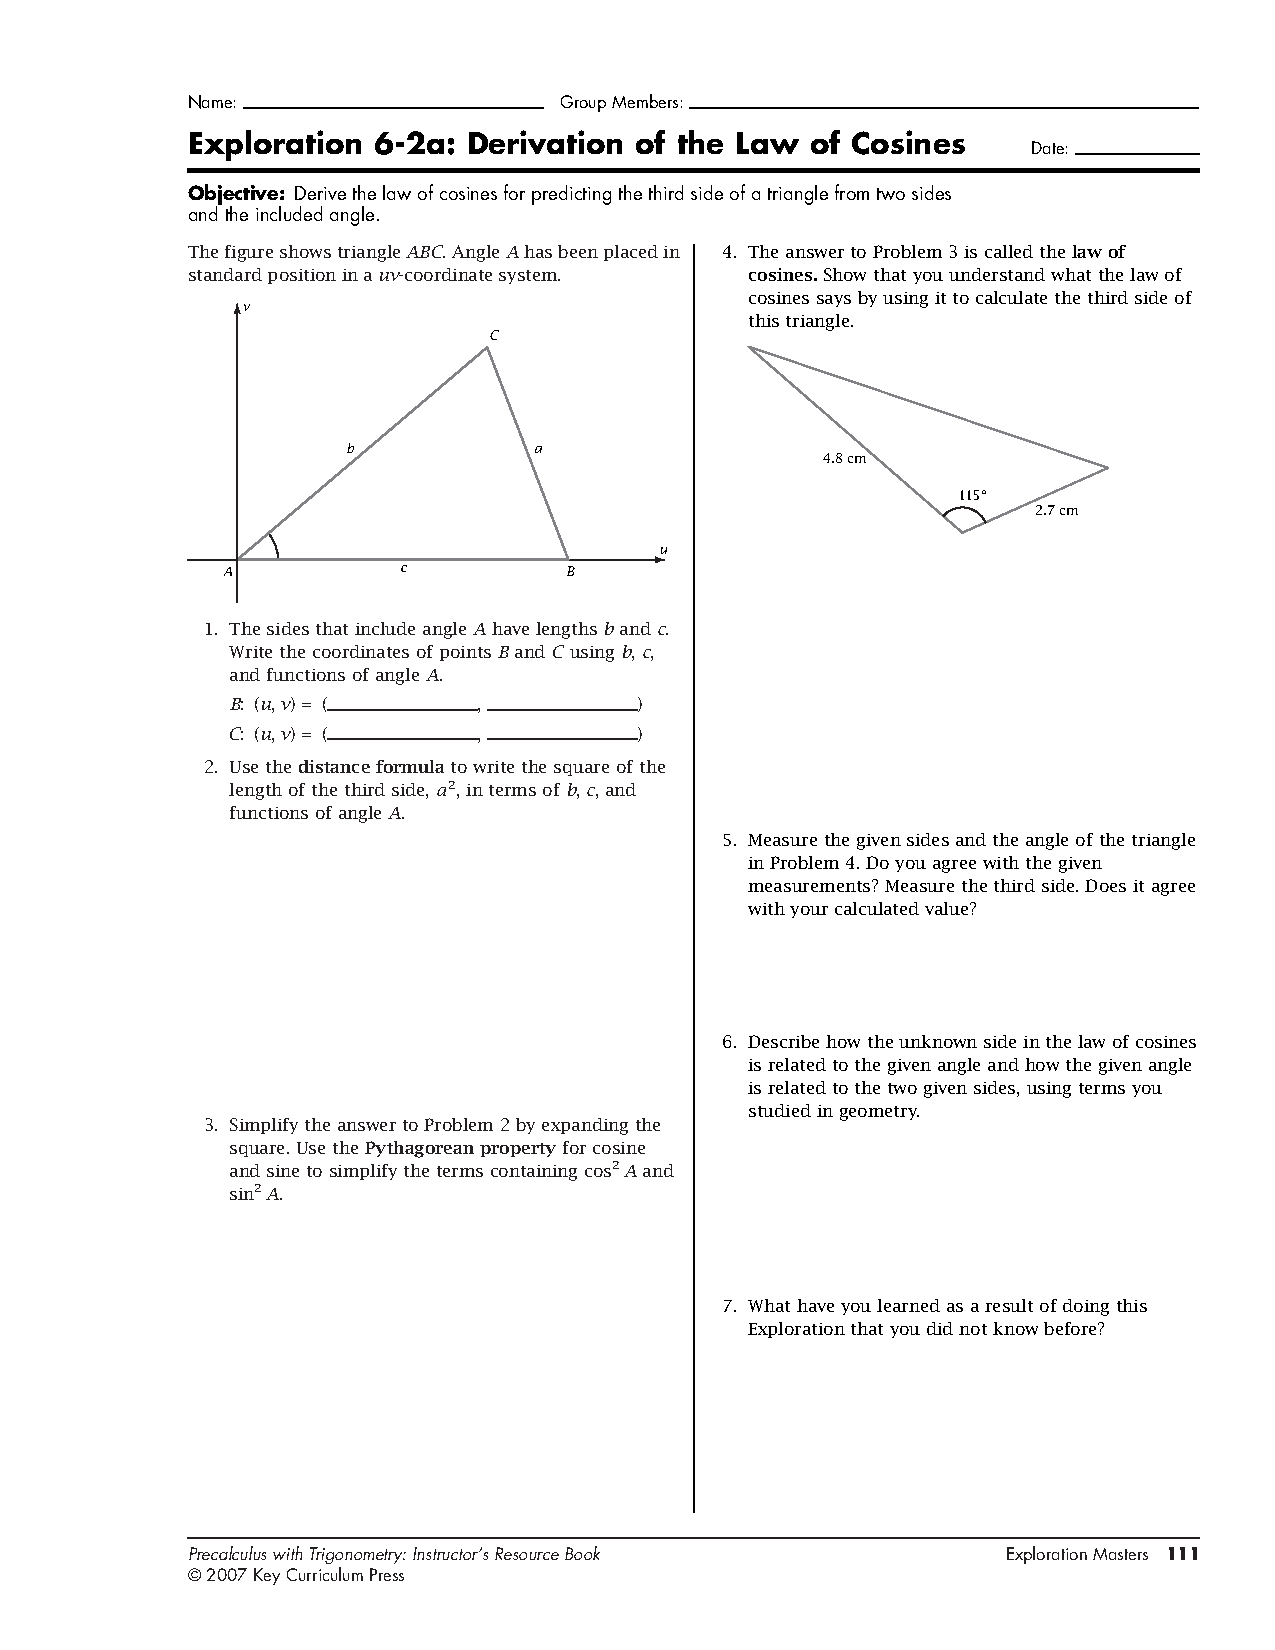
\includegraphics[width=\paperwidth]{ch11/1102p.pdf}}
\newpage
\subsection{SSS}
\subsection{SAS}
\newpage
\subsection{Exercises}
to be done in kuta

%									11 - 3
\newpage
\invisiblesection{Law of Sines}
\subsection{Problems}
\noindent\makebox[\textwidth]{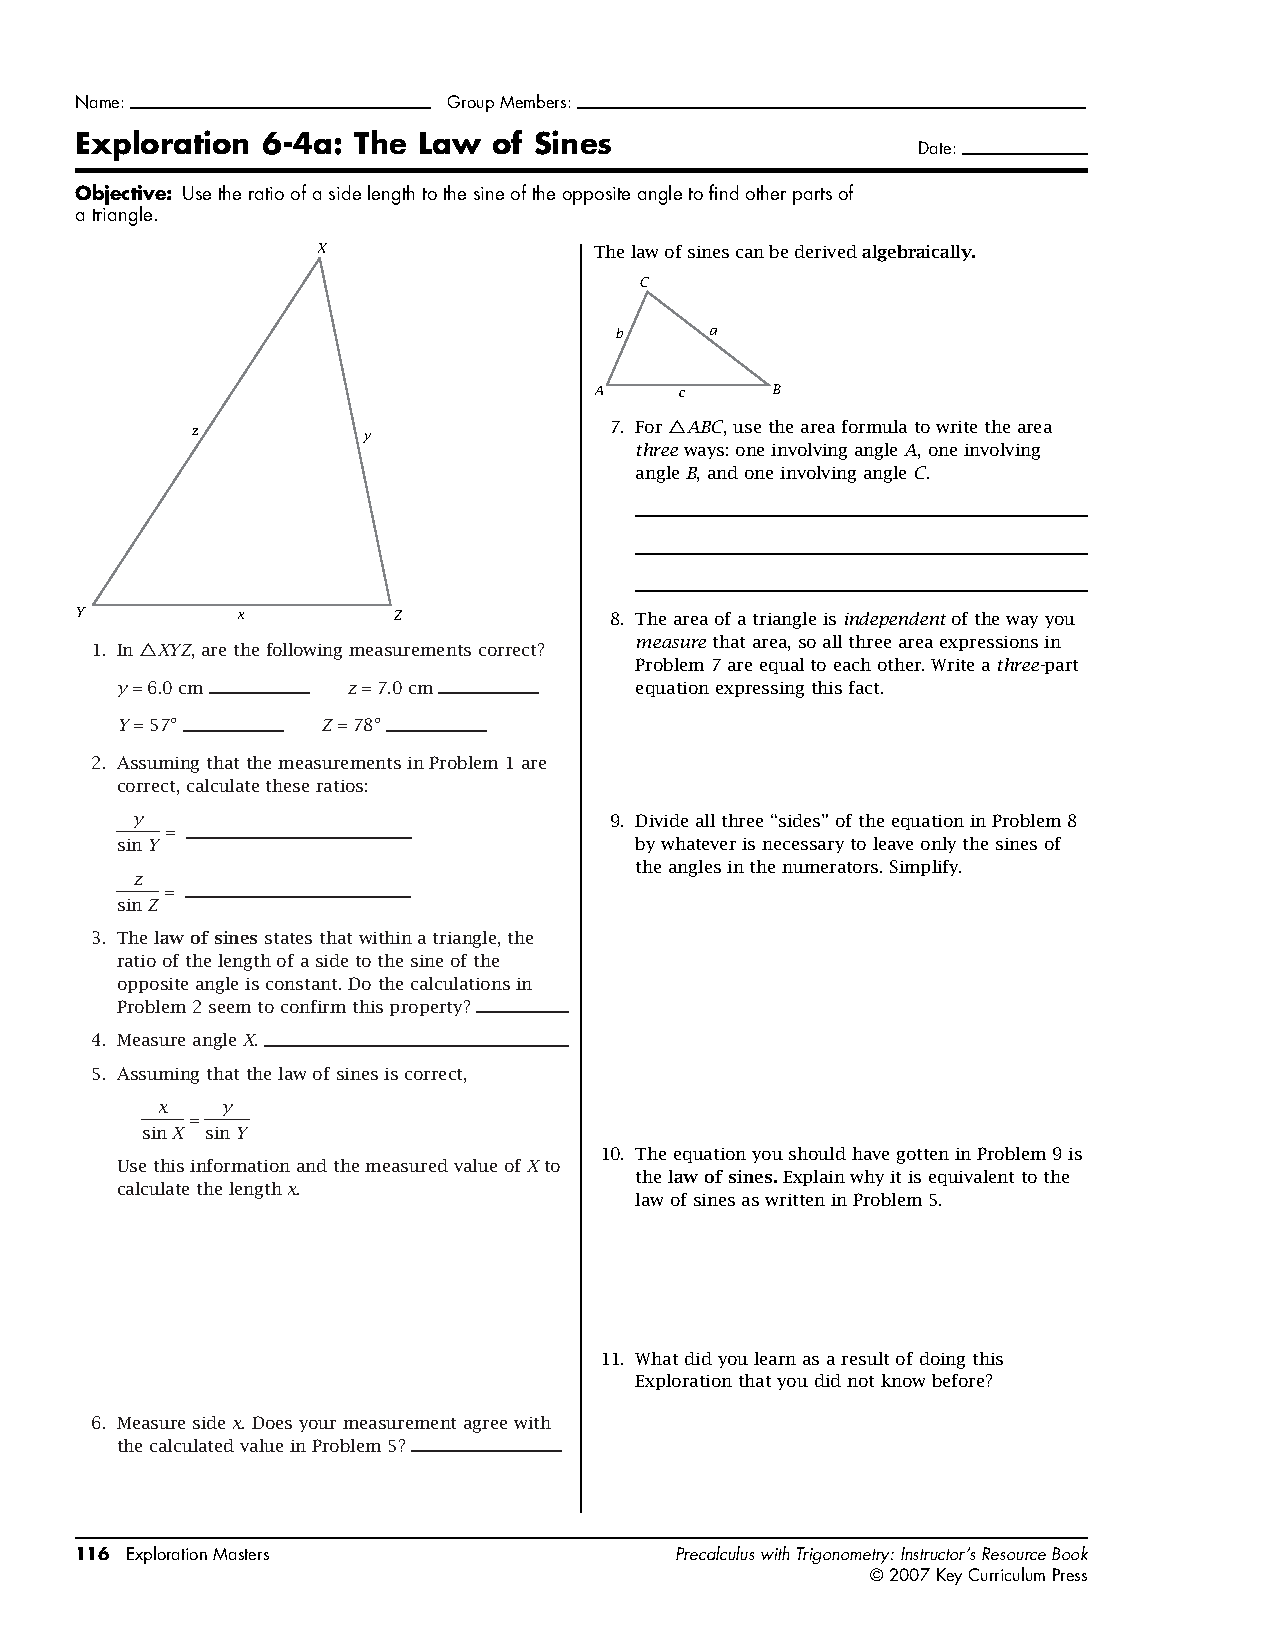
\includegraphics[width=\paperwidth]{ch11/1103p.pdf}}
\newpage
\subsection{Imagining the Height}
\subsection{SAA}
\subsection{ASA}
\newpage
\subsection{Exercises}
to be done in kuta

%									11 - 4
\newpage
\invisiblesection{The Ambiguous Case}
\subsection{Problems}
\noindent\makebox[\textwidth]{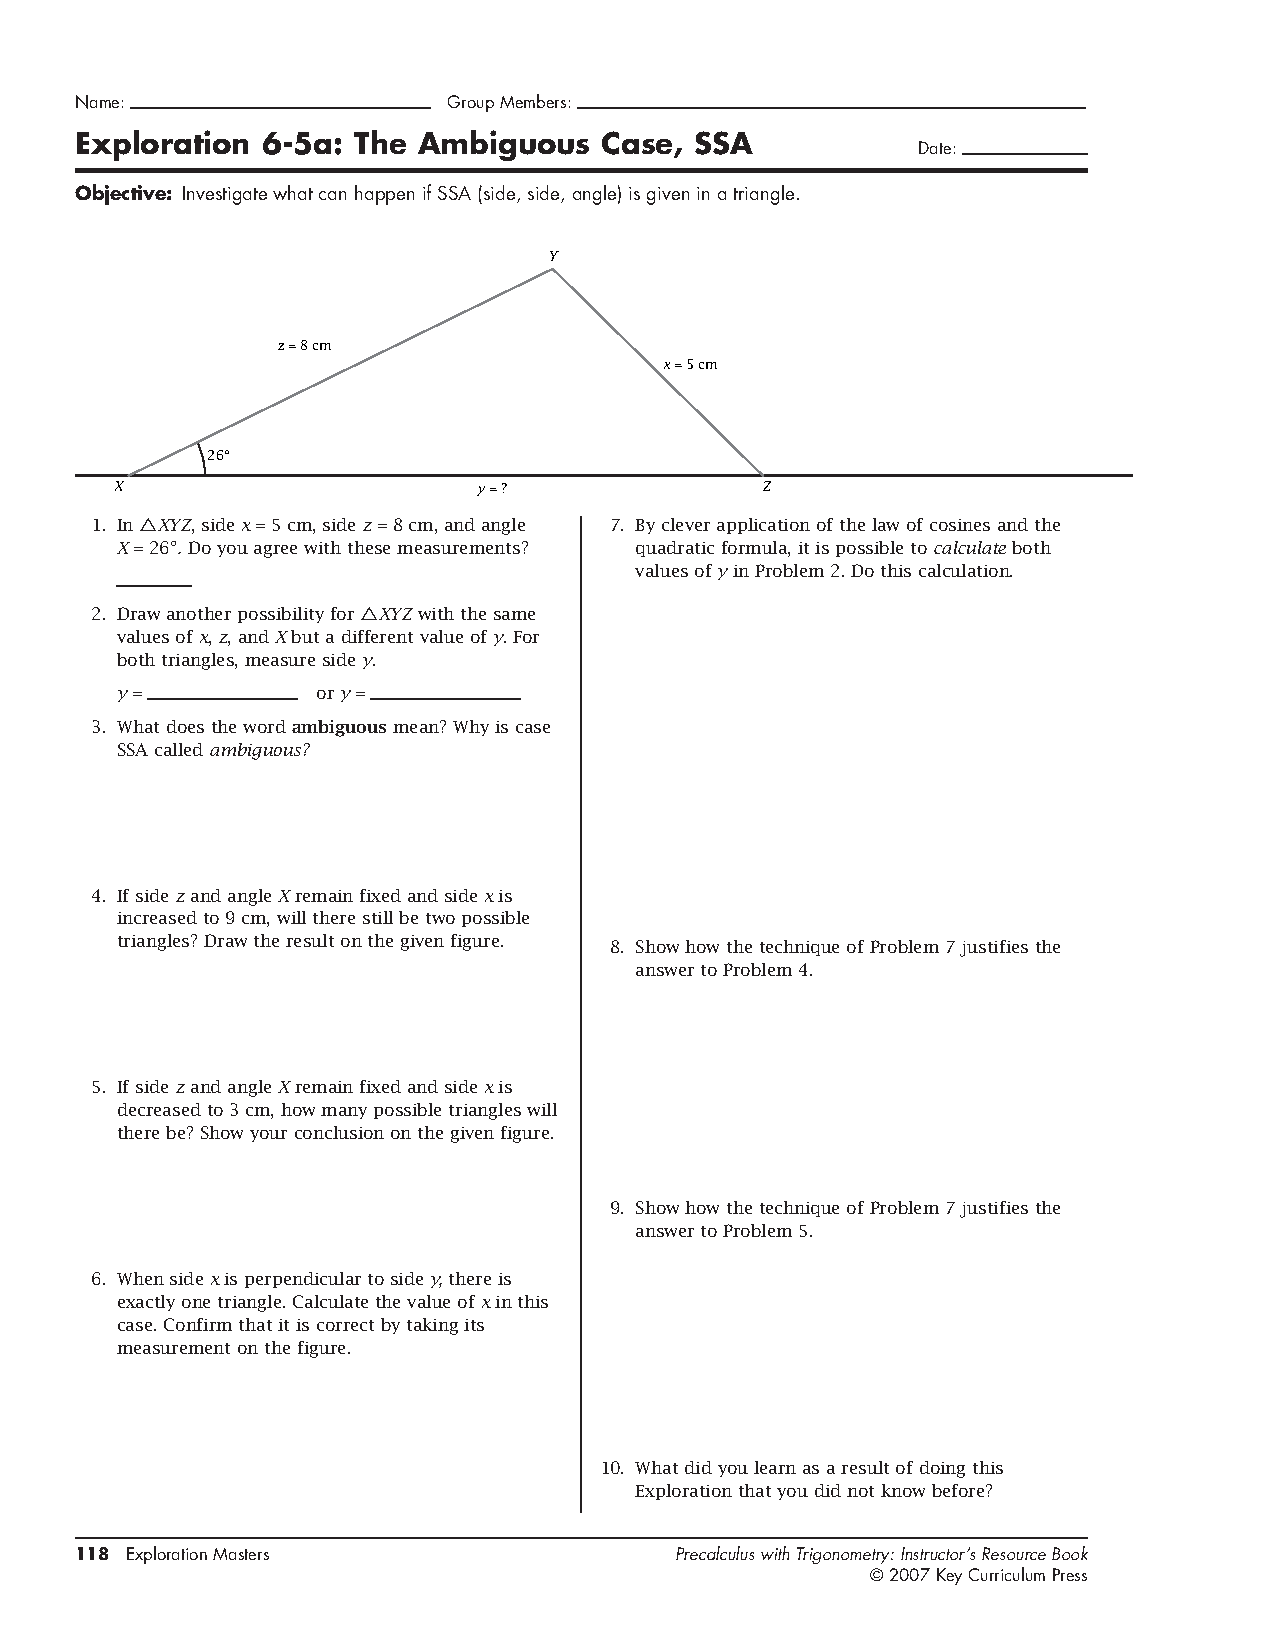
\includegraphics[width=\paperwidth]{ch11/1104p.pdf}}
\newpage
\subsection{SSA}
\subsection{Related Rates}
\subsection{Exercises}
to be done in kuta


%									11 - 5
\newpage
\invisiblesection{2D Vectors}
\subsection{Problems}
\noindent\makebox[\textwidth]{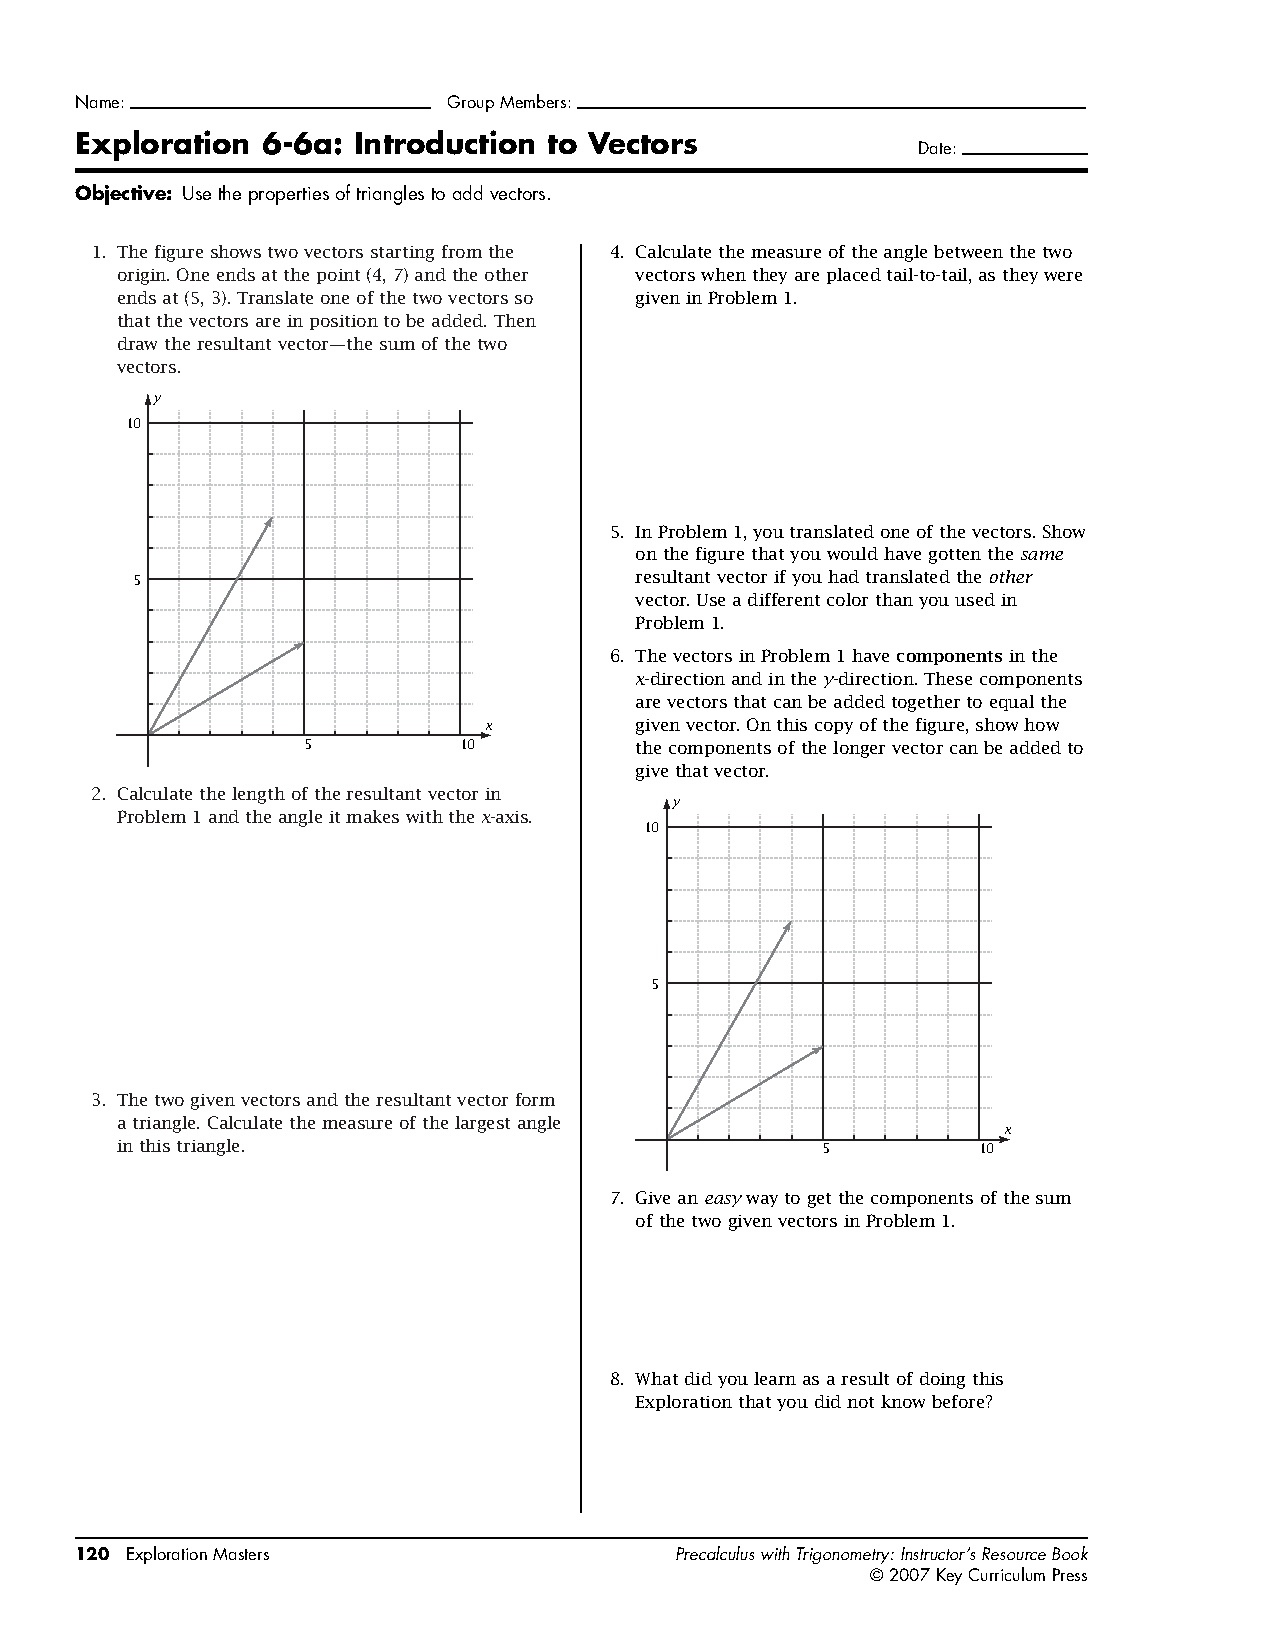
\includegraphics[width=\paperwidth]{ch11/1105p.pdf}}
\newpage
\subsection{Definition and Magnitude}
Vectors have a length, called their magnitude, written with absolute value bars.
\index{Absolute Value!of vectors}
\subsection{Vector Components}
\subsection{Heading and Bearing}
\newpage
\subsection{Exercises}
to be done in kuta

%									11 - 6
\newpage
\section{Review}
\subsection{Chapter Review}
\subsection{Chapter Test}